\documentclass[tikz,border=6pt]{standalone}
\usepackage{amsmath,amssymb}
\usepackage{xcolor}
\definecolor{accent}{HTML}{A13D2C}
\definecolor{accent2}{HTML}{2B5F6B}
\definecolor{muted}{HTML}{5A564F}
\definecolor{panel}{HTML}{F8F6F0}
\definecolor{linecol}{HTML}{D8D2C4}
\definecolor{astroblue}{HTML}{1B4F72}
\definecolor{sunyellow}{HTML}{E8A33D}
\definecolor{colthree}{RGB}{60,140,80}
\usetikzlibrary{calc,arrows.meta,plotmarks}
\IfFileExists{results/ch12/lane_emden_n3.dat}{\def\datadir{results/ch12/}}{\def\datadir{../results/ch12/}}
\begin{document}
% Regimes of pressure in the (log T, log rho) plane, SI units. Boundaries:
%  light = gas:            rho = (a mu mH / 3 kB) T^3,          mu = 0.62  -> log rho = -19.72 + 3 log T
%  degenerate = classical: E_F(nonrel) = kB T, mu_e = 2         -> log rho = -4.915 + 1.5 log T
%  relativistic electrons: p_F = m_e c, mu_e = 2                -> rho = 1.96e9
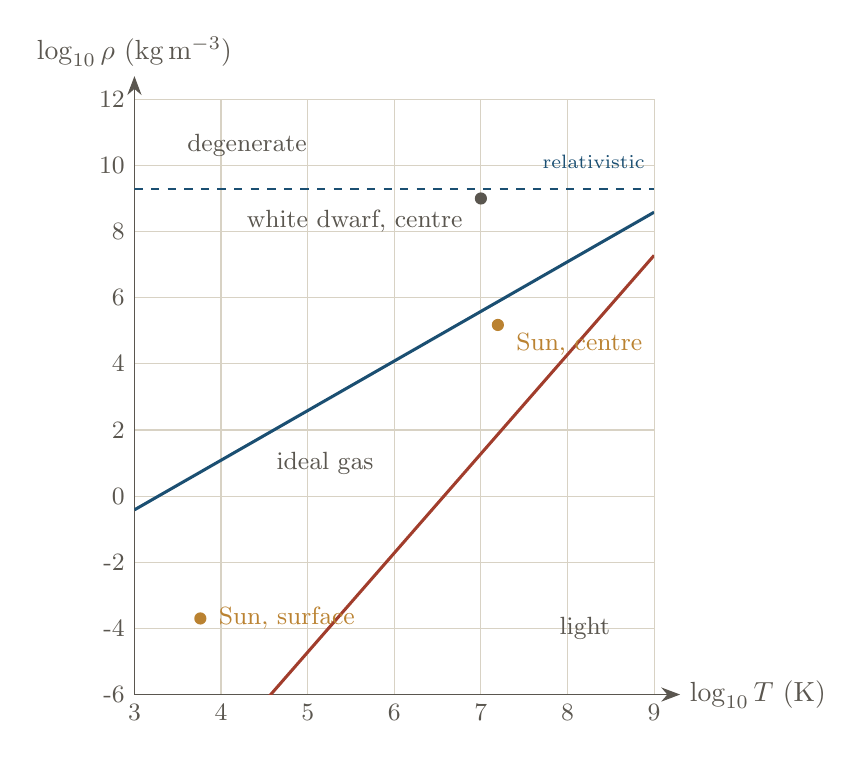
\begin{tikzpicture}[x=1.1cm,y=0.42cm, >={Stealth[length=2.4mm]}]
  \draw[linecol] (3,-6) grid[xstep=1,ystep=2] (9,12);
  \draw[->, muted] (3,-6) -- (9.3,-6) node[right] {$\log_{10}T\ (\mathrm K)$};
  \draw[->, muted] (3,-6) -- (3,12.7) node[above] {$\log_{10}\rho\ (\mathrm{kg\,m^{-3}})$};
  \foreach \x in {3,...,9} \node[below, muted] at (\x,-6) {\small \x};
  \foreach \y in {-6,-4,...,12} \node[left, muted] at (3,\y) {\small \y};
  \begin{scope}
    \clip (3,-6) rectangle (9,12);
    \draw[accent, line width=1.1pt, domain=4.5:9] plot (\x, {-19.72 + 3*\x});
    \draw[astroblue, line width=1.1pt, domain=3:9] plot (\x, {-4.915 + 1.5*\x});
    \draw[astroblue, dashed, line width=1.0pt] (3,9.29) -- (9,9.29);
  \end{scope}
  \node[muted, align=center] at (5.2,1.0) {\small ideal gas};
  \node[muted] at (8.2,-4.0) {\small light};
  \node[muted] at (4.3,10.6) {\small degenerate};
  \node[astroblue, right] at (7.6,10.1) {\scriptsize relativistic};
  \fill[sunyellow!80!black] (7.196,5.176) circle[radius=2.2pt];
  \node[sunyellow!80!black, right] at (7.296,4.576) {\small Sun, centre};
  \fill[sunyellow!80!black] (3.761,-3.699) circle[radius=2.2pt];
  \node[sunyellow!80!black, right] at (3.861,-3.699) {\small Sun, surface};
  \fill[muted] (7,9) circle[radius=2.2pt];
  \node[muted, left] at (6.9,8.3) {\small white dwarf, centre};
\end{tikzpicture}
\end{document}
